% !TeX root = ../thuthesis-example.tex

\chapter{\MakeUppercase{NUIX-Studio network and computational performance tests}}

Evaluating how devices are created and how simultaneous work is performed in the IoT-VR environment is an important part of this research. This chapter describes several experiments used for testing the NUIX-Studio platform's performance.

\section{Testing equipment preconfiguration}

There are several devices in the example configuration (Figure~\ref{fig:TestingEquipment-figure}):
\begin{enumerate}
    \item A Smart Wi-Fi lamp;
    \item A PC running openHAB server and the NUIX-Studio App instance;
    \item A PC running the NUIX-Studio App instance;
    \item An Oculus Quest VR Headset;
    \item A smart vacuum cleaner.
\end{enumerate}

\begin{figure}
  \centering
  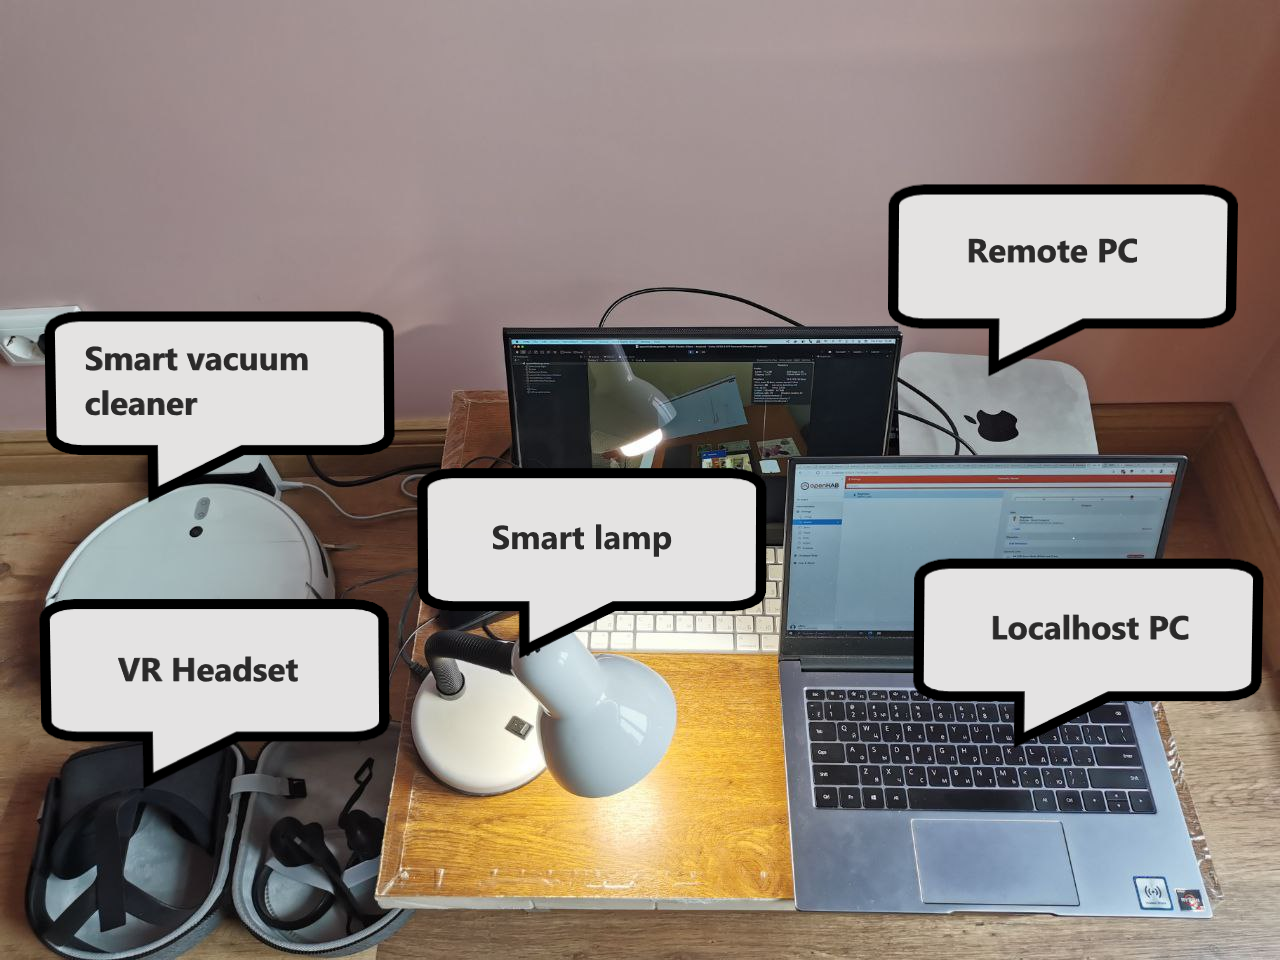
\includegraphics[width = 0.9 \linewidth]{figures/TestingEquipment.png}
  \caption{Testing equipment.}
  \label{fig:TestingEquipment-figure}
\end{figure}

In the initial experiment, gesture control functionality is added to the smart lamp\footnote{a Smart vacuum cleaner and a remote PC will be used in the next experiments} by creating Tags for Light and Gesture Recognition Widgets in the virtual environment scene (Figure~\ref{fig:ItemEditPage-figure}). In other words, the virtual lamp light is equivalent to the real-world one, and a gesture control interface is implemented. To test the system functioning, a VR-IoT platform user performs three actions:

\begin{enumerate}
    \item Put on Virtual reality headset;
    \item Press the virtual button to establish a Client-Server connection and receive the items list;
    \item Perform a ``Thumbs up'' gesture. By rotating one's fist, the lamp brightness changes in the VR-IoT environment\footnote{In both the real and virtual worlds.} (Figure~\ref{fig:FullBrightnessOculus-figure}).
\end{enumerate}

\begin{figure}
  \centering
  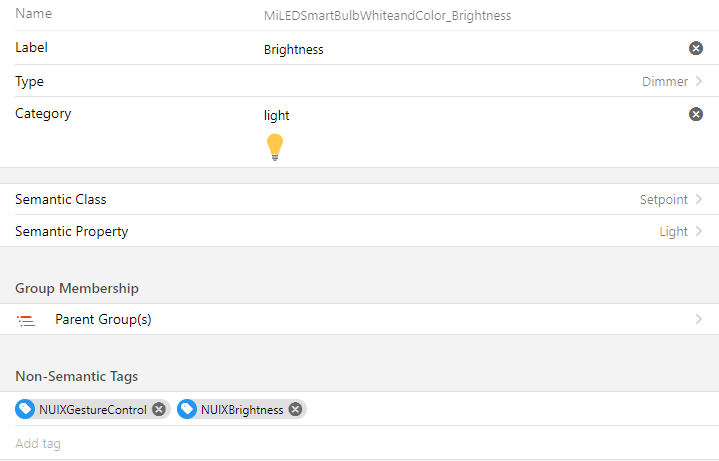
\includegraphics[width = 0.9 \linewidth]{figures/ItemEditPage.png}
  \caption{Item Edit Page.}
  \label{fig:ItemEditPage-figure}
\end{figure}


\begin{figure}
  \centering
  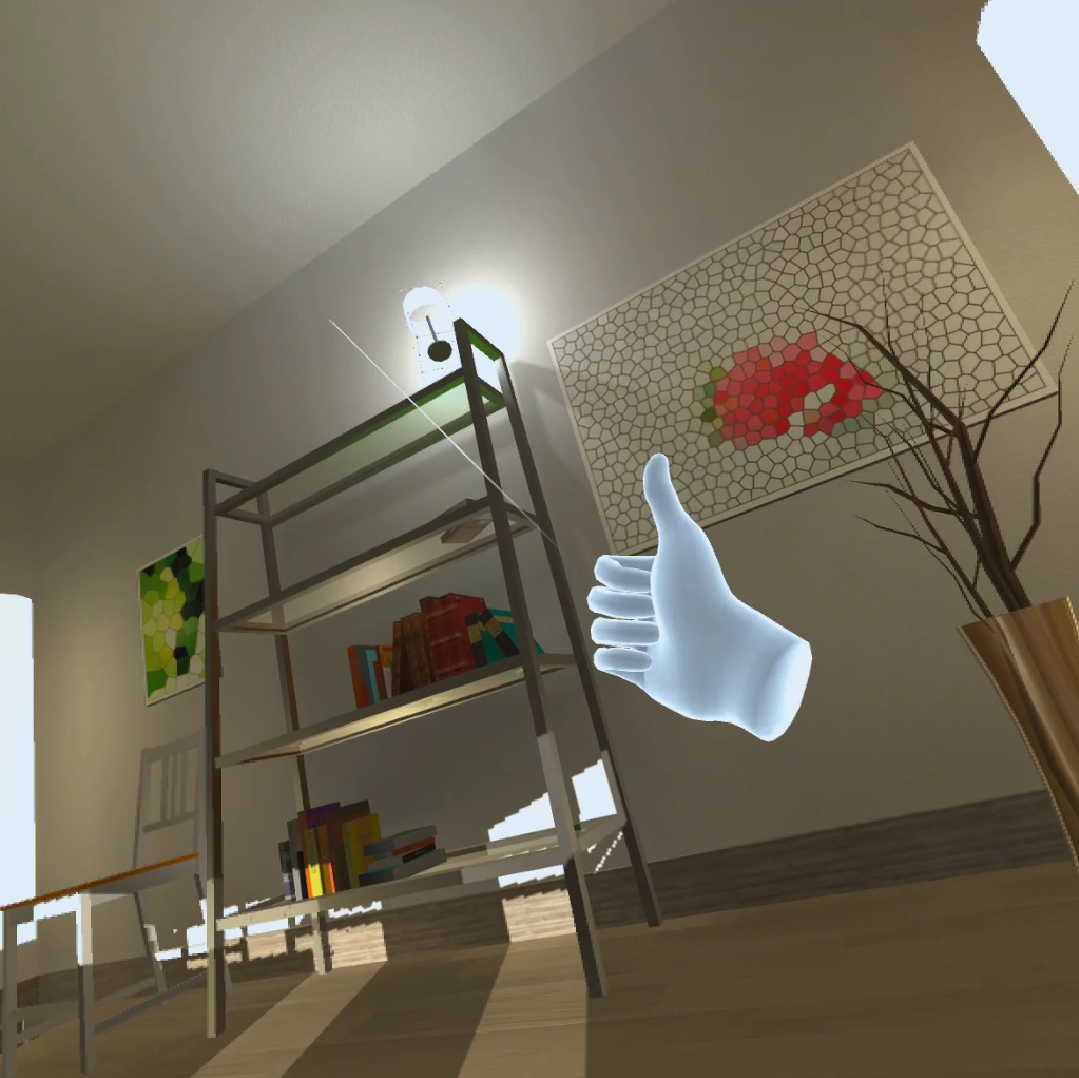
\includegraphics[width = 0.6 \linewidth]{figures/FullBrightnessOculus.png}
  \caption{``Thumbs up'' gesture.}
  \label{fig:FullBrightnessOculus-figure}
\end{figure}

The user of the platform performed these actions\footnote{In this experiment, the platform developer was the user.} (Figure~\ref{fig:BrightnessControl-figure}). Thus, support for gestures was added to control the lamp's brightness. The experiment to create a new device for the existing environment can be considered a success.

\begin{figure}
  \centering
  \subcaptionbox{Lamp brightness set to ~75\%\label{fig:HalflBrightness}}
    {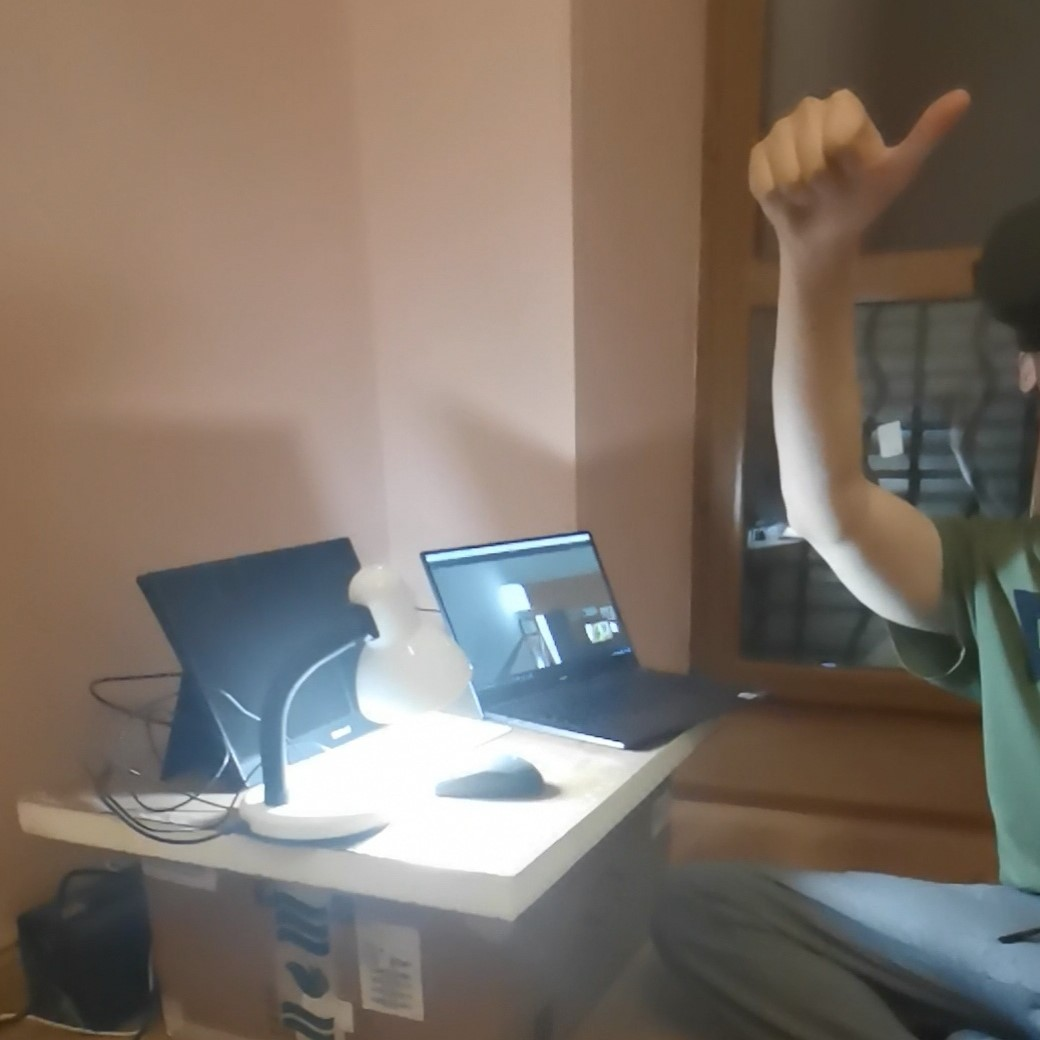
\includegraphics[width=0.45\linewidth]{figures/HalflBrightness.jpg}}
  \subcaptionbox{Lamp brightness set to 100\%\label{fig:FullBrightness}}
    {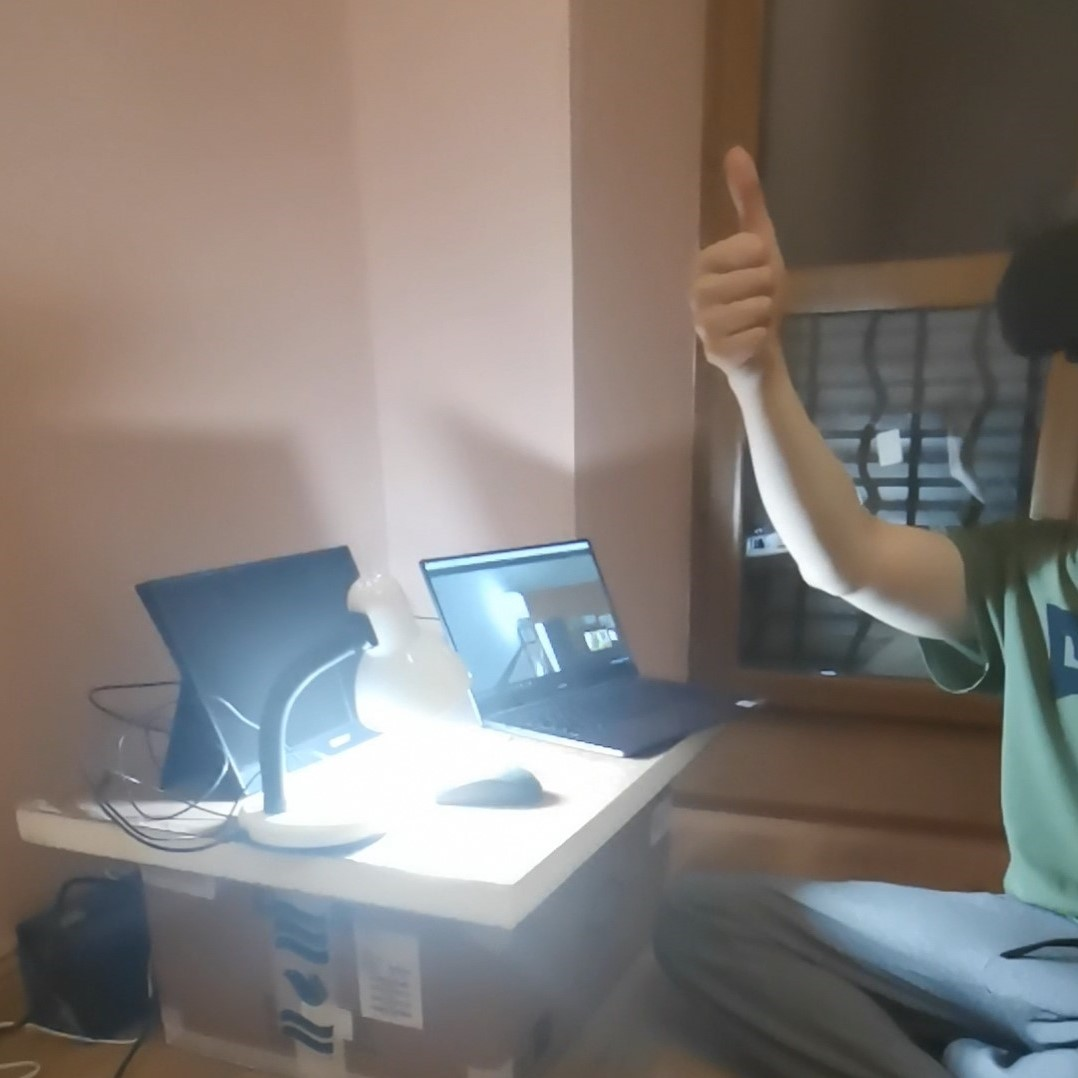
\includegraphics[width=0.45\linewidth]{figures/FullBrightness.jpg}}
  \caption{Experiment of the lamp brightness control. In both cases the real lamp and the NUIX-Studio App virtual lamps on the Local PC and on Oculus Quest have the same brightness value.}
  \label{fig:BrightnessControl-figure}
\end{figure}

\section{System startup and event processing time measurements}

The first experiment is a system startup analysis, performed on three devices by registering the startup time (Figure~\ref{fig:SystemStartupScheme-figure}). The hardware specifications are listed in Table~\ref{tab:hardware-specifications-table}~\footnote{A Localhost PC is a notebook running the openHAB server as well as one instance of NUIX-Studio App; A Remote PC is a computer running one instance of the NUIX-Studio App and connected to the same Wi-Fi network as the localhost PC; Oculus Quest is a Virtual Reality Headset running the NUIX-Studio APP and connected to the same Wi-Fi network as the PCs.}.

\begin{figure}
  \centering
  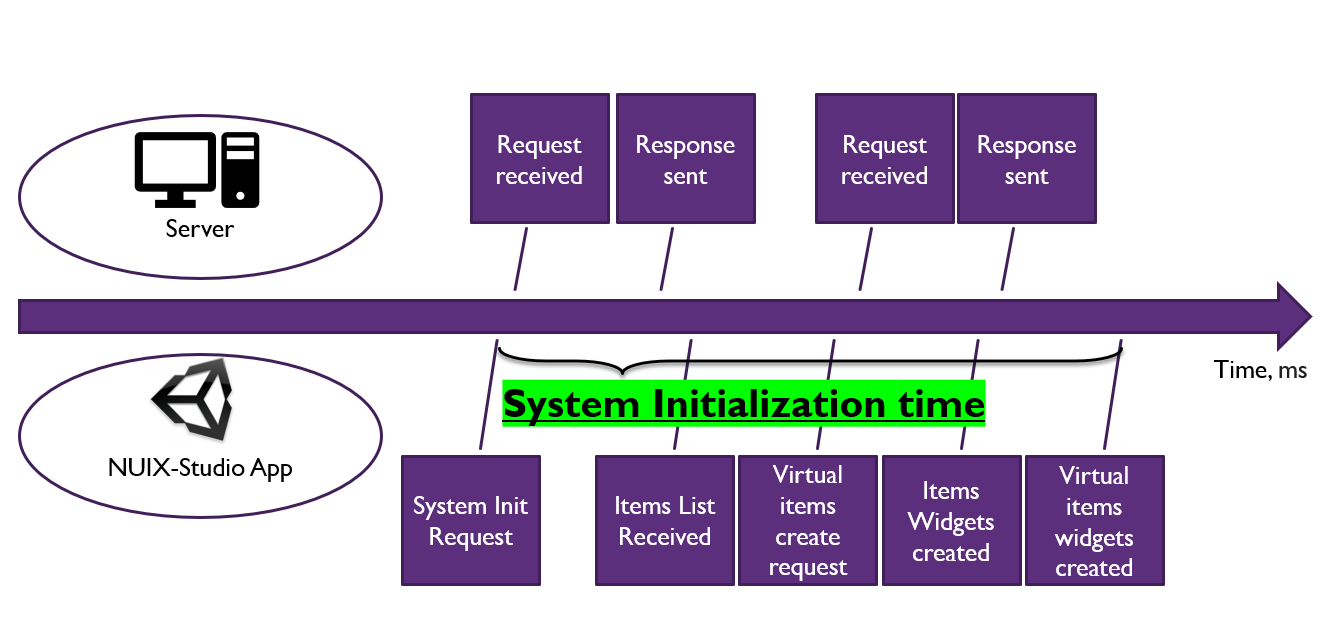
\includegraphics[width = 0.9 \linewidth]{figures/SystemStartupScheme.png}
  \caption{System startup scheme.}
  \label{fig:SystemStartupScheme-figure}
\end{figure}

\begin{table}
  \centering
  \begin{threeparttable}[c]
    \caption{Hardware specifications in the experimental setup}
    \label{tab:hardware-specifications-table}
    \begin{tabular}{ll}
      \toprule
      Unit    &         Specifications                 \\
      \midrule
      Localhost PC & Ryzen 5 3500u, Windows 10 \\
      Remote PC & Core i5 4278U, macOS 11.2.3    \\
      Oculus Quest        & Qualcomm Snapdragon 835, Android-based            \\
      \bottomrule
    \end{tabular}
  \end{threeparttable}
\end{table}

Each test was performed on a new Unity App instance to avoid caching influence. Then, mean values for the tests were calculated. As seen in Figure~\ref{fig:SystemInitTime-figure}, the system initialization is a time-consuming operation, on average taking from 200ms to over 600ms to perform.

\begin{figure}
  \centering
  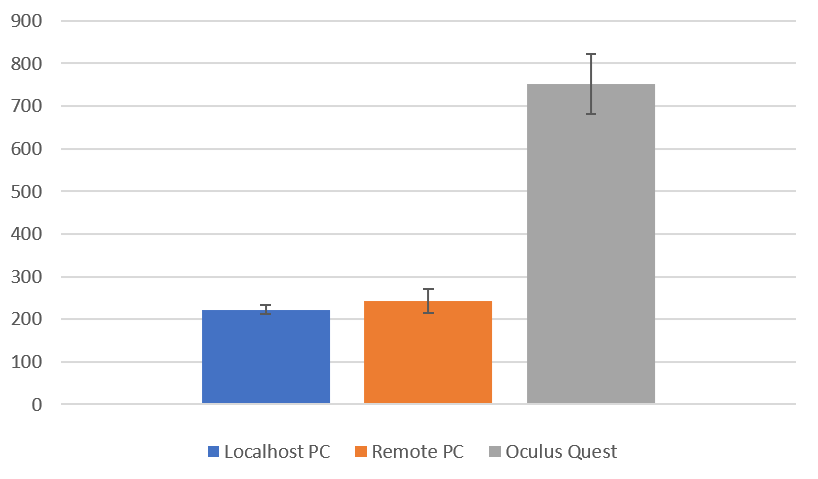
\includegraphics[width=0.9\linewidth]{figures/SystemInitTime.png}
  \caption{System initialization time measured on different client devices, in ms}
  \label{fig:SystemInitTime-figure}
\end{figure}

In the next experiment, the event processing time was measured. On one of the devices running the NUIX-Studio App instance, a user changed an Item value \footnote{In this case, the brightness of the smart bulb was changed by moving the corresponding pinch slider widget}. The server processed the received request to change the Item parameter, and then an Event containing information about the new Item value was sent to all devices connected to the server. The device on which this Item change occurred ignored the new incoming value because it was equal to the old value. Next, the processing time of a request on another device was estimated (Figure~\ref{fig:EventProcessingScheme-figure}).

\begin{figure}
  \centering
  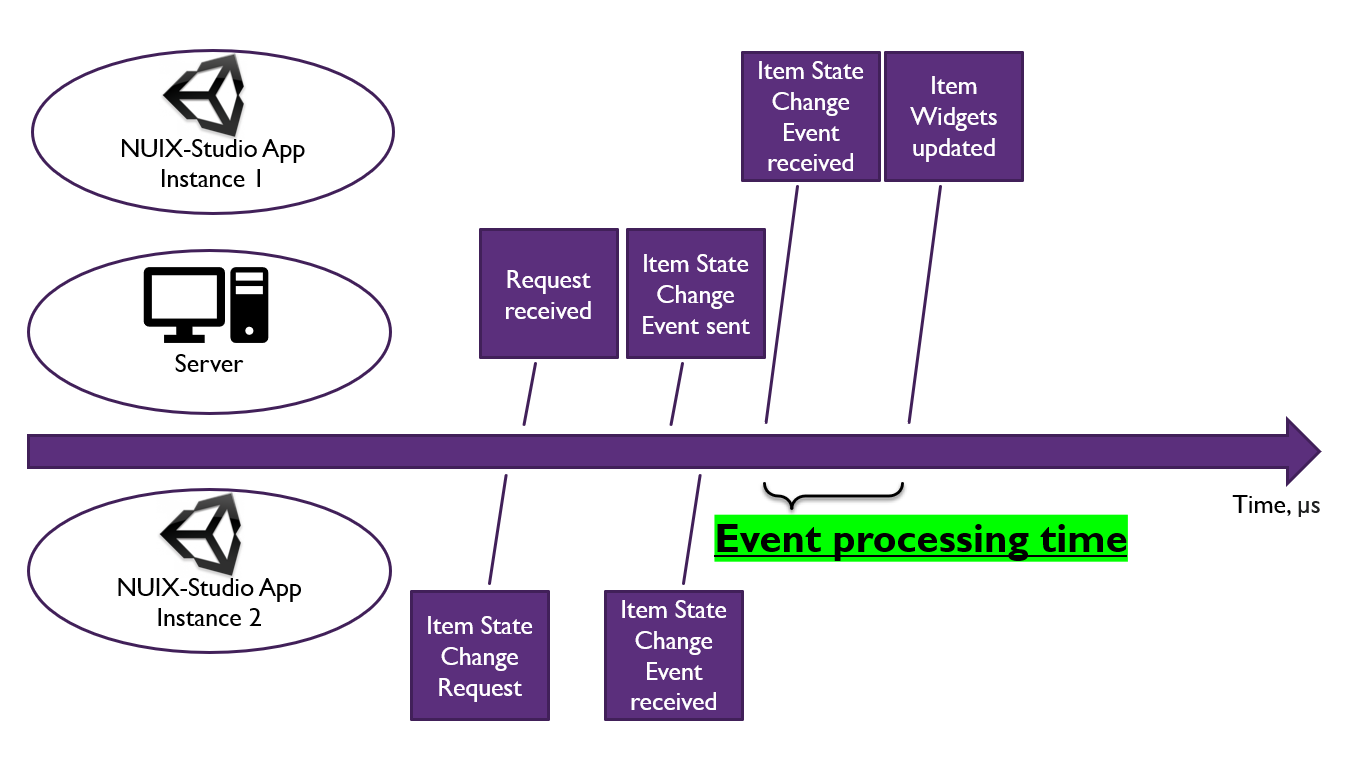
\includegraphics[width = 0.9 \linewidth]{figures/EventProcessingScheme.png}
  \caption{Event processing scheme.}
  \label{fig:EventProcessingScheme-figure}
\end{figure}

As seen on the resulting histogram (Figure~\ref{fig:EventProcessingTime-figure}), Oculus Quest's performance on this test was outstanding. The processing time difference can be explained by the fact that the NUIX-Studio App runs in an unoptimized state on Windows and macOS\footnote{Unity editor mode}, but can run significantly faster after the App instances are built for the platforms.

\begin{figure}
  \centering
  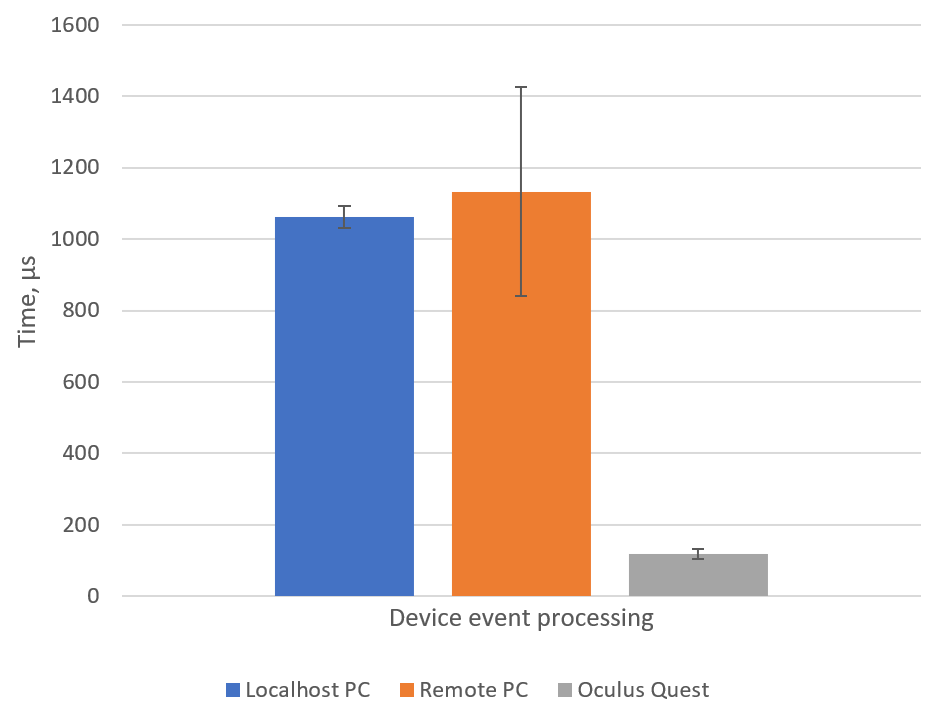
\includegraphics[width = 0.9 \linewidth]{figures/EventProcessingTime.png}
  \caption{Event Processing time measured on different devices, in \textmu{}s}
  \label{fig:EventProcessingTime-figure}
\end{figure}

The results of this experiment will be used in the future. System initialization time is based on the device hardware performance. In some later experiments, it is better not to include system initialization in time calculations. Event processing time is relatively low for each device and can be ignored in most cases.

\section{Testing complex computations}

The analysis of platform performance is not the study's primary goal, but it helps with finding bottlenecks. The following experiment shows that it is viable to perform rendering tasks on a separate server. The experiment equipment includes a Virtual reality headset, a smart light bulb, and a server running an application on it. For instance, a light sensor is used inside a Smart home environment, located at a relatively large distance from the lamp (2-3 meters), and is triggered when the amount of light falling on its sensor exceeds a certain threshold. For example, this setup can be used in industry to provide a comfortable lighting level while maintaining an optimal amount of energy consumption. The light sensor is triggered precisely at a sufficiently large value of the lamp brightness. Hence, the sensor must adjust to the brightness level of the light bulb very accurately.

The previous experiment showed that gesture control could be used to adjust a lamp's brightness level. This experiment shows that the transfer of computations from the Virtual reality headset to the server is necessary for specific scenarios. The user is asked to perform the same steps as in the previous experiment, with one more step added:  setting the brightness to the specified level. In this experiment, the light sensor is triggered at a lamp light brightness level of 50 out of 100 \footnote{Using Fitts' law, it can be assumed that setting up brightness levels to different values takes different amounts of time. However, this effect is considered not significant for the experiment.}. The user's task is to set the light brightness to the specified value as quickly as possible using gesture control. In order to omit additional operations not related to the direct use of gestures (such as starting the system), the user had to repeat the step by setting the brightness of the light to the specified value twice. The interval between the first and second times, when the lamp brightness is equal to the specified value, can be divided into two components (Equation \eqref{eq:totaltime}): the user reaction time to a successful change in the brightness level $ t_{react} $, and the execution time of the new calibrations $ t_{cal} $.


\begin{equation}
  t = t_{react} + t_{cal}
  \label{eq:totaltime}
\end{equation}

Two people participated in the two series of the experiment. In the first series, the light's illumination was computed on a Virtual reality headset, and in the second, on a server that was periodically calculating the lightmap. User reaction time $ t_{react} $ is a value independent of the changed synchronization parameters. Therefore, the difference in calculated time in the first and the second series of the experiment is equal to the difference in time spent on calibrating the lamp brightness in the experiment (Equation \eqref{eq:deltatime}).

\begin{equation}
  t _{\Delta} = (t_{react} + t_{cal_1}) - (t_{react} + t_{cal_1}) = t_{cal_1} - t_{cal_2}
  \label{eq:deltatime}
\end{equation}

As can be seen in the Figure~\ref{fig:ExperimentTime-figure}, the time it took the participants to perform the task is unstable, but on average, it took both users more time to perform the task in the first series than in the second series. In Figure~\ref{fig:DeltaTime-figure} it can be seen that $t_{\Delta}$ is more than zero for most observations.

\begin{figure}
  \centering
  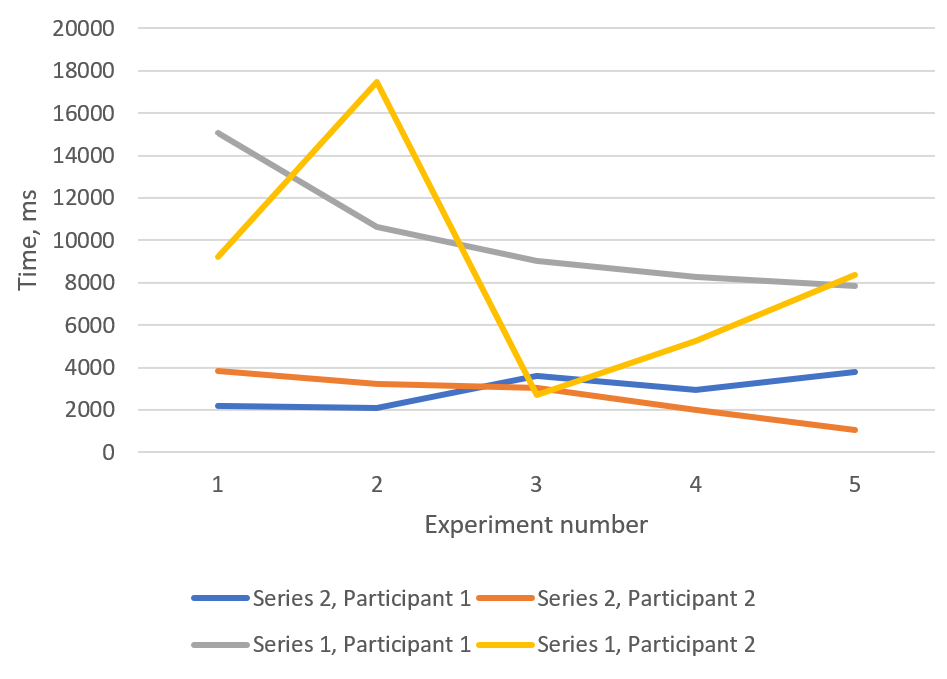
\includegraphics[width = 0.9 \linewidth]{figures/ExperimentTime.png}
  \caption{Time spent on calibrating the lamp brightness, in ms}
  \label{fig:ExperimentTime-figure}
\end{figure}


\begin{figure}
  \centering
  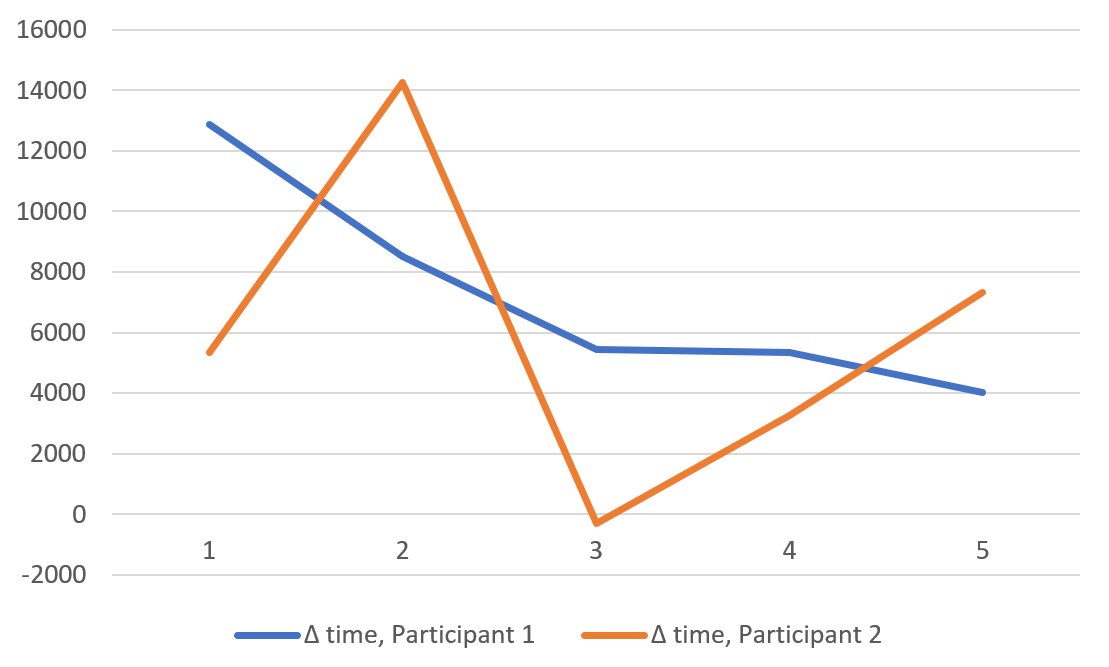
\includegraphics[width = 0.9 \linewidth]{figures/DeltaTime.png}
  \caption{The difference between the time spent on calibrating the lamp brightness in the first and the second series of the experiment, in ms}
  \label{fig:DeltaTime-figure}
\end{figure}

Additional data were analyzed during the experiment, such as the number of frames per second with which the NUIX-Studio App was rendered on the screen (Figure~\ref{fig:exp-screenshot}). Figure~\ref{fig:Series2FPSpng-figure} shows that in the first series of the experiment, the number of frames per second drops significantly as soon as the system is initialized and the Widgets for the Items from the Semantic model are created. In the second series of the experiment, such a drop is no longer observed (Figure~\ref{fig:Series1FPSpng-figure}). Because the illumination was computed on a separate device, the number of frames per second drops only slightly \footnote{Probably because illumination computation significantly impacts the device's performance, especially its Graphics processing unit.}.

\begin{figure}
  \centering
  \subcaptionbox{Series 1\label{fig:exp-screenshot-a}}
    {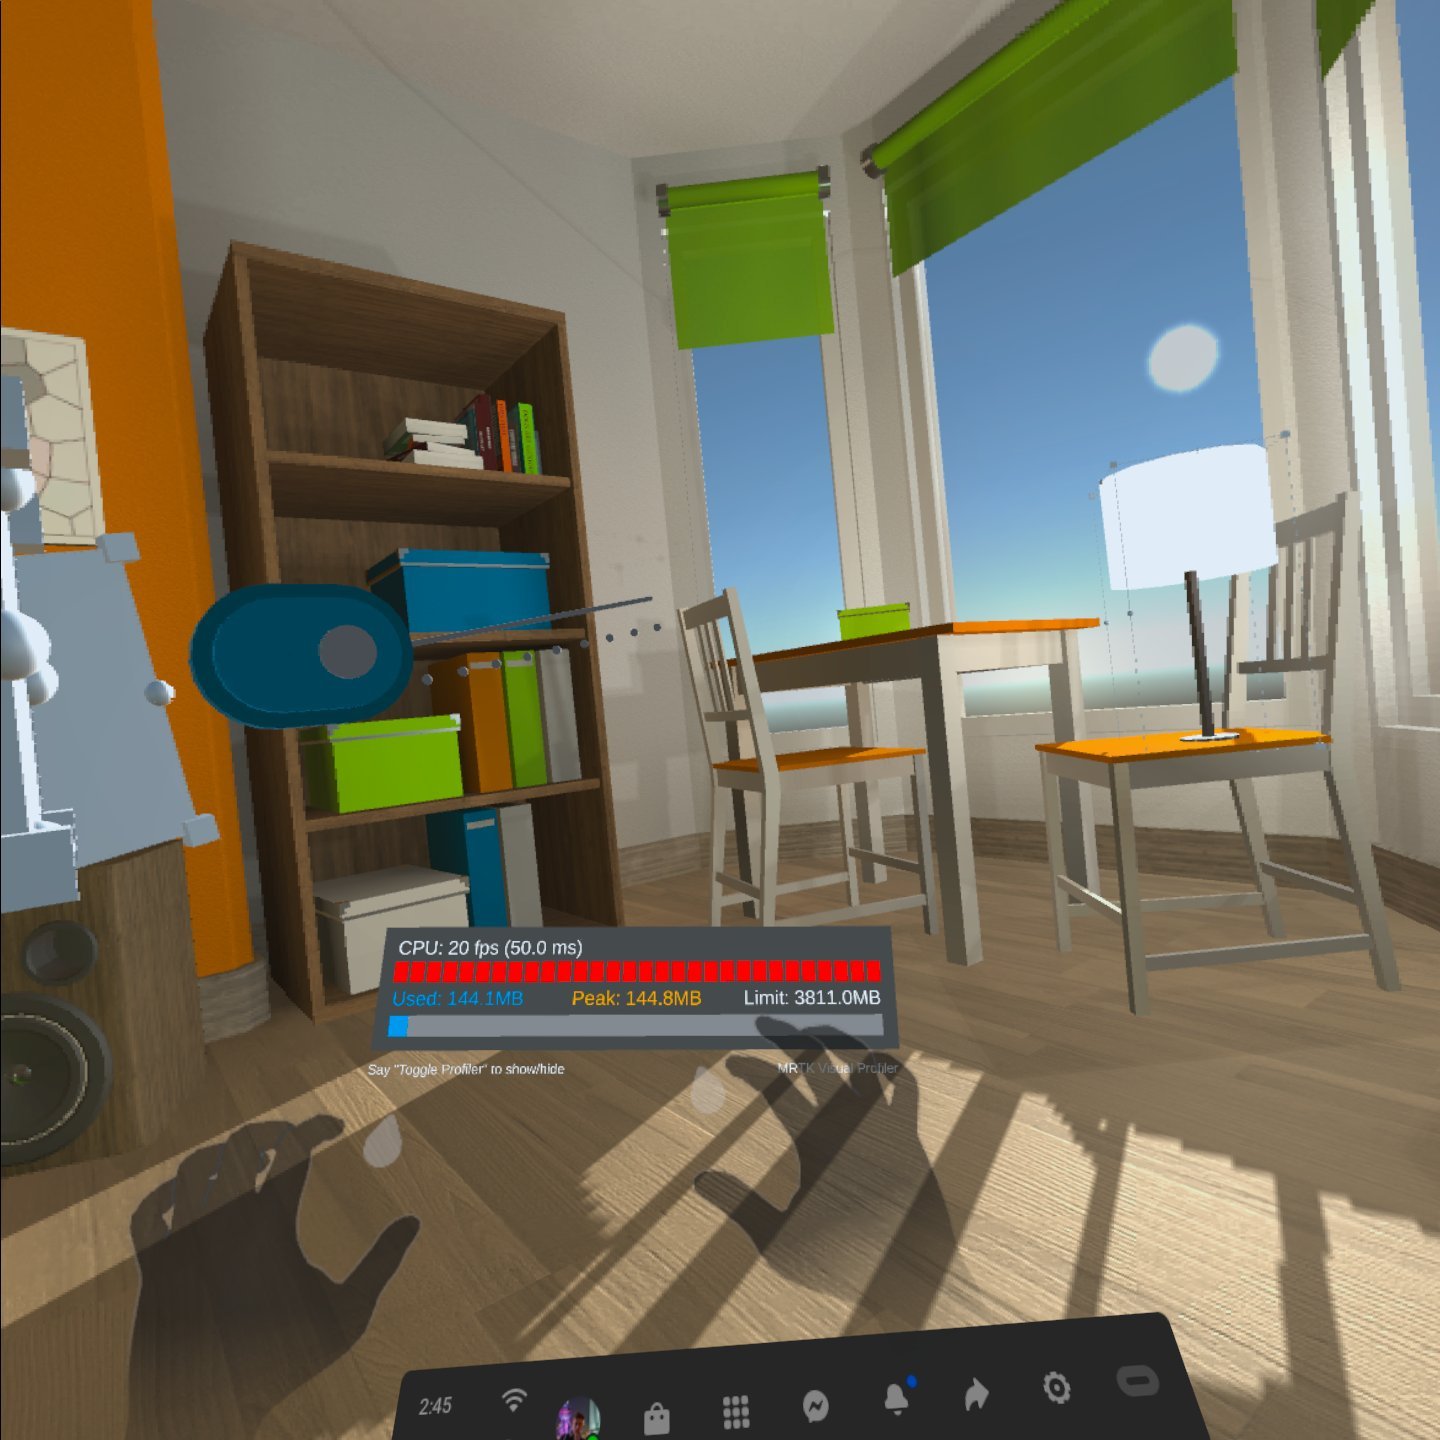
\includegraphics[width=0.45\linewidth]{figures/Series1FPSOculus.jpg}}
  \subcaptionbox{Series 2\label{fig:exp-screenshot-b}}
    {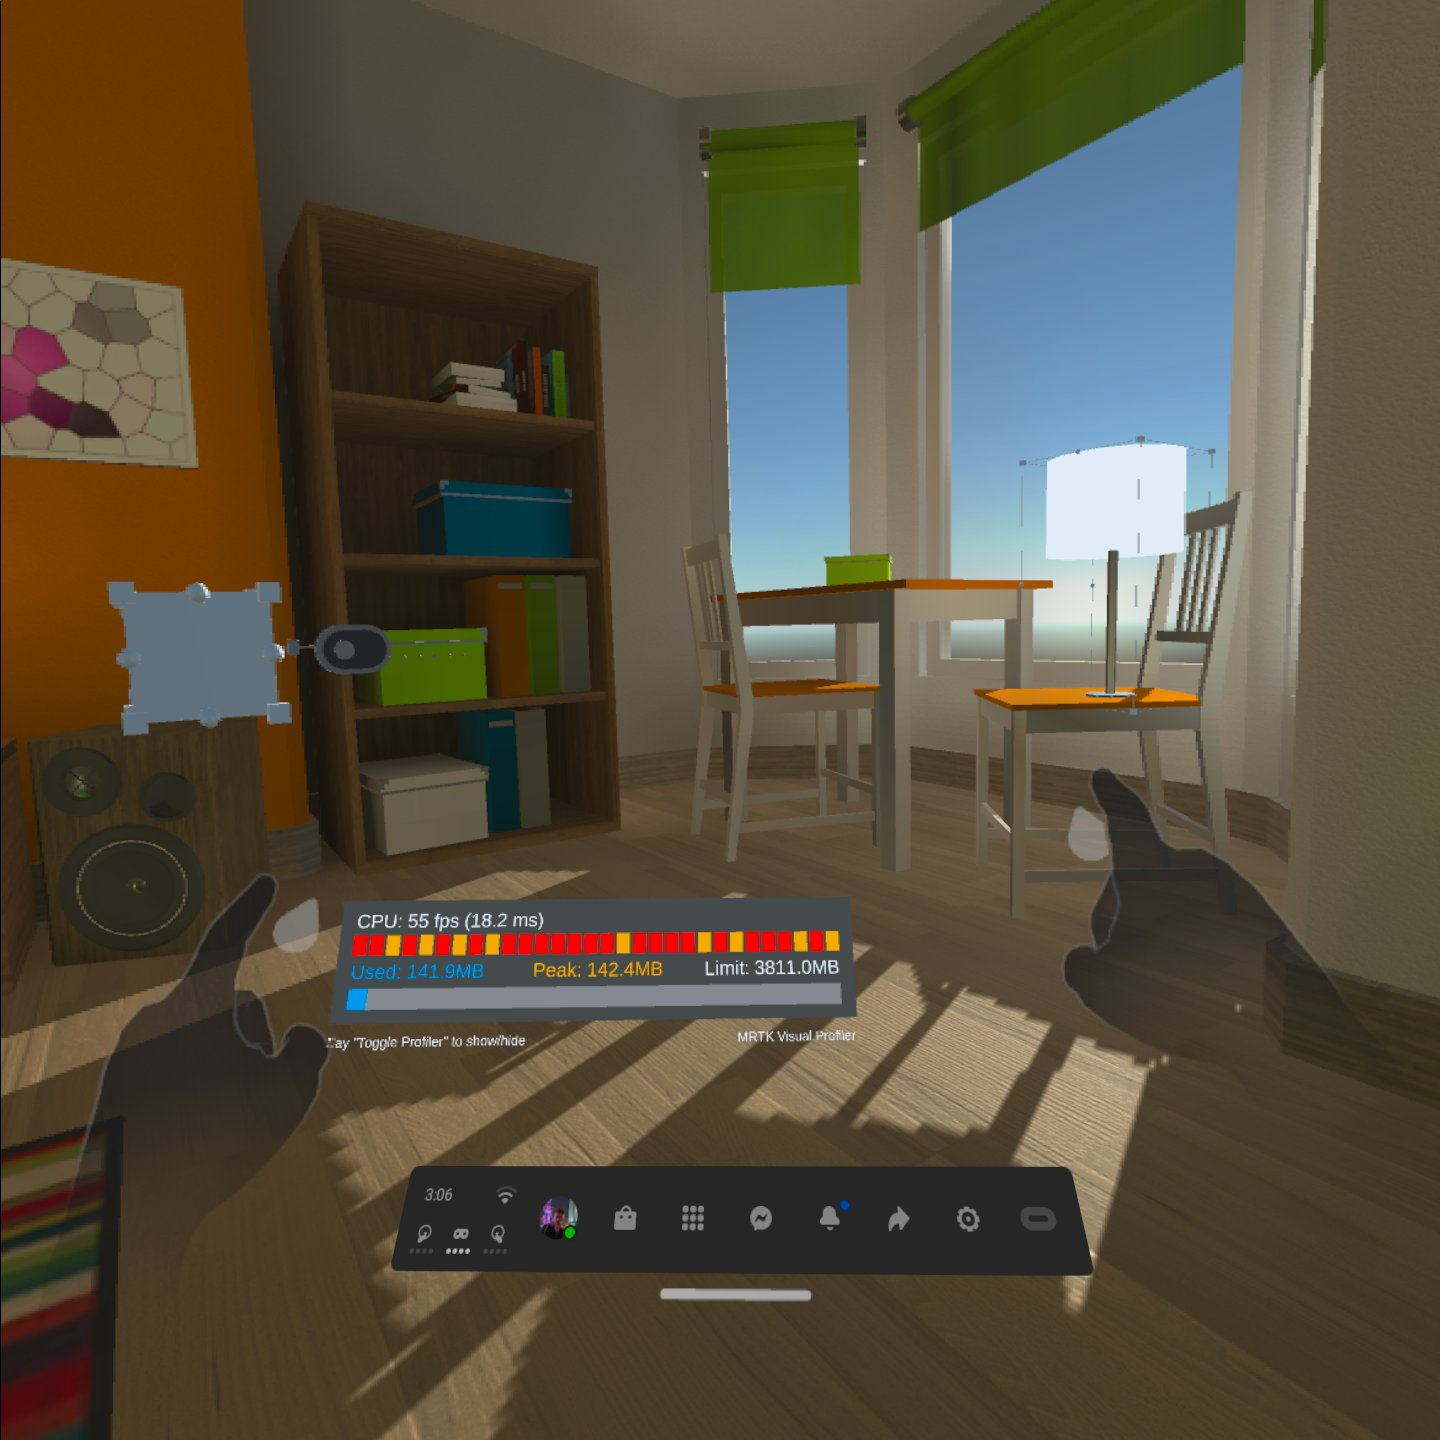
\includegraphics[width=0.45\linewidth]{figures/Series2FPSOculus.jpg}}
  \caption{Screenshots of the experiment.}
  \label{fig:exp-screenshot}
\end{figure}

\begin{figure}
  \centering
  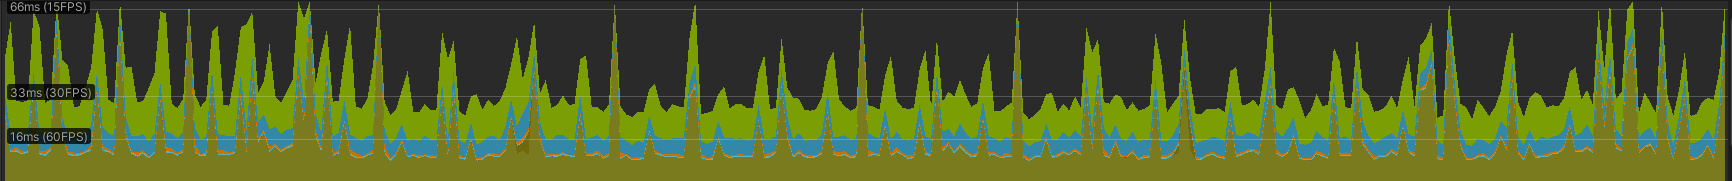
\includegraphics[width = 0.9 \linewidth]{figures/Series2FPSpng.png}
  \caption{FPS graph during the first series of the experiment on computation transfer.}
  \label{fig:Series2FPSpng-figure}
\end{figure}

\begin{figure}
  \centering
  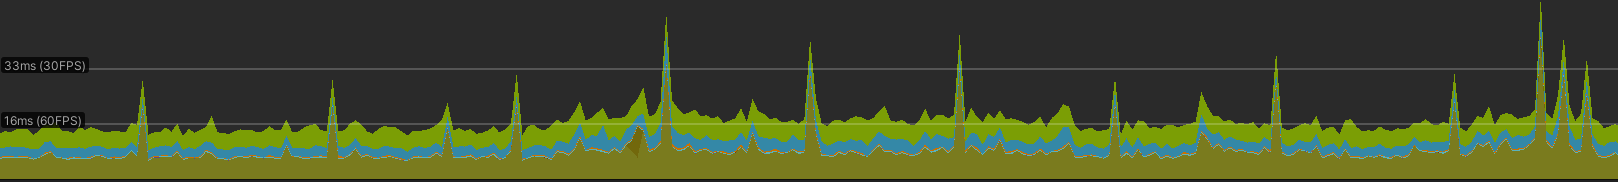
\includegraphics[width = 0.9 \linewidth]{figures/Series1FPS.png}
  \caption{FPS graph during the second series of the experiment on computation transfer.}
  \label{fig:Series1FPSpng-figure}
\end{figure}

Considering that gesture recognition is processed no more than once per frame, it significantly influenced the user experience, resulting in a big $t_{\Delta}$. The frequency of gesture value retrieval can be called a polling rate. When a polling rate is 1000Hz, the gesture position is retrieved once every millisecond (Table~\ref{tab:polling-rate-table}). There is probably a linear dependency between the time spent on performing the calibration and the polling rate during the test.

\begin{table}
\let\TPToverlap=\TPTrlap
  \centering
  \begin{threeparttable}[c]
    \caption{Polling rate to response time of gesture recognition dependence}
    \label{tab:polling-rate-table}
    \begin{tabular}{@{}p{\textwidth}@{}}
    \centering
    \begin{tabular}{ll}
      \toprule
      Polling rate, Hz    & Response time, ms                 \\
      \midrule
      72Hz & 13.9ms \\
      65Hz & 15.4ms \\
      20Hz & 50ms \\
      10Hz & 100ms \\
      \bottomrule
    \end{tabular}
    \end{tabular}
  \end{threeparttable}
\end{table}

However, the experiment's main challenge was to show how transferring resource-intensive computing from a VR headset to a server improves the user experience because this is significant for the VR-IoT Research platform. Thus, the experiment can be considered successful.\footnote{Please note that this experiment cannot be considered scientifically substantiated since the number of tests and the number of participants was relatively small. In addition, it was impossible to control external factors that add random error, such as system optimization (which affects the stability of the frame rate), room lighting (which affects the accuracy of hand recognition), the size of the participants' hands, and the participants' experience with virtual reality systems. As a result, reproducing this experiment is almost impossible. Nevertheless, this experiment serves as an example of the need to transfer resource-intensive computing from the VR headset to the server.}

\section{Testing simultaneous work scenarios}

In the experiment, the author demonstrated that it is possible to work together in one VR-IoT environment by adding new IoT devices to the system and changing their parameters:
\begin{enumerate}
    \item The time for adding a device to the system is limited by the performance of a specific platform and the speed of the Internet connection within the Wi-Fi network. When running 300 sequential ping tests from a remote PC to a localhost PC, all the values ​​obtained were less than 100ms, with 90 percent of the values ranging from 45ms to 70ms. The time spent by the device on creating widgets for a smart vacuum cleaner roughly corresponded to the time of system initialization;
    \item Time interval from changing an Item on the remote PC to updating the widgets on localhost PC did not exceed 60ms.
\end{enumerate}

Thus, the speed of the network plays a significant role in the operation of the system. The minimal network latency available now can be significantly reduced in future Wi-Fi~6 networks and 6G networks, significantly improving the simultaneous work inside the same VR-IoT environment. However, it has been observed that operations such as adding new devices to the system will remain time-consuming. Since there is a request to create Unity Game Objects for each of the Item's widgets, the author assumes that the main delay is associated precisely with the internal processes inside the Unity 3D engine. The delays connected to hand recognition will continue to decrease, since every new generation of Virtual Reality headsets has a higher refresh rate screens compared to the previous ones. 

The NUIX-Studio application is provided in the next chapter. Several hypotheses connected to research in AIoT-VR have been tested with the help of the VR-IoT platform. 